\chapter{Resultados}\label{cap:resultados}
\FloatBarrier
\section{Organización y alcance de la evidencia}
Este capítulo presenta los resultados del clasificador de radiografías y del controlador neuronal que aproxima la política MPC. La exposición sigue la secuencia experimental del capítulo anterior: evaluación en computador, conversión y compilación, validación numérica en la STM32N6570-DK y pruebas de integración. Se incorpora una comparación complementaria con NUCLEO-L476RG, que cierra el capítulo. Para radiografías, se estudian la clasificación y el costo de inferencia; para MPC, se añade el comportamiento de la planta simulada en lazo cerrado. La comparación permite examinar qué parte del beneficio de cuantizar el modelo se conserva después de implementarlo.

La evidencia experimental comprende predicciones, matrices de confusión, registros de ST Edge AI, grafos de los modelos, listados de instrucciones y ocho ensayos HIL \cite{res_archivo2026}. La campaña complementaria comprende validaciones QAT del clasificador en STM32N6 y registros de NUCLEO-L476RG para ambos casos de estudio \cite{res_ampliacion2026}. Las tablas y figuras sintetizan las mediciones y los cálculos derivados de estos registros. En el análisis se distingue entre resultados medidos, magnitudes calculadas e interpretación de los hallazgos.

\begin{table}[htbp]\centering\small
\caption{Conjuntos de evidencia utilizados y alcance de cada comparación.}\label{tab:res_alcance}
\begin{tabularx}{\linewidth}{p{3.5cm}p{2.6cm}Y}\toprule
Evaluación & Muestras & Resultado que permite examinar\\\midrule
Radiografías en PC & 624 imágenes & Clasificación, concordancia y recursos del archivo\\
Radiografías con ST & 8 imágenes & Fidelidad de la implementación y perfil de inferencia\\
Demostración UART & 16 imágenes & Recepción, ejecución y respuesta de la aplicación\\
MPC en simulación & 200 estados iniciales & Cumplimiento del criterio de lazo cerrado\\
MPC con ST & 200 entradas & Concordancia numérica por inferencia y perfil\\
MPC en HIL & 8 ensayos; 100 acciones cada uno & Trayectorias, restricciones y tiempos UART/inferencia\\\bottomrule
\end{tabularx}
\fuente{registros experimentales}
\end{table}

Los conjuntos de ocho, dieciséis y 624 radiografías se interpretan por separado. De igual forma, las 200 entradas utilizadas en la validación ST no son las 200 condiciones iniciales de las simulaciones: la primera prueba compara salidas para entradas aisladas; la segunda evalúa trayectorias de 16 s. Las ocho condiciones HIL constituyen una selección determinista y no una repetición de toda la campaña de simulación.

El tamaño del archivo exportado, los pesos compilados y el búfer de activaciones se presentan como magnitudes diferentes. Las cifras de memoria de red no incluyen necesariamente todo el programa, la pila, el transporte UART o los datos de la aplicación. Tampoco se convierten los tiempos en consumo energético, puesto que los archivos no contienen mediciones eléctricas de estas ejecuciones.

\begin{table}[htbp]\centering\small
\caption{Cobertura de evaluación por variante y destino.}\label{tab:cobertura_variantes}
\begin{tabularx}{\linewidth}{Ycccc}\toprule
Caso y variante & PC & N6 CPU & \shortstack{Ruta N6\\Neural-ART} & L476\\\midrule
Radiografías Float32 & Sí & ND & ND & ND\\
Radiografías PTQ INT8 & Sí & Sí & Sí & Fallo\\
Radiografías QAT INT8 & Sí & Sí & Sí & Sí\\
Radiografías INT16x8 & Sí & Sí & Sí$^{*}$ & ND\\
Radiografías Mixed-3 & Sí & ND & ND & ND\\
Radiografías Mixed-5 & Sí & Sí & Sí & Fallo\\\midrule
MPC Float32 & Sí & Sí & ND & ND\\
MPC PTQ INT8 por tensor & Sí & Sí & Sí & Sí\\
MPC PTQ INT8 por canal & Sí & Sí & Sí & Sí\\
MPC QAT INT8 & Sí & Sí & Sí & Sí\\
MPC INT16x8 & Sí & Sí & ND & Sí\\
MPC precisión mixta & Sí & Sí & Sí & Sí\\\bottomrule
\end{tabularx}
\fuente{evaluaciones en PC y registros de validación ST de la campaña}
\par\smallskip\footnotesize El asterisco señala una ruta INT16x8 cuya ejecución nativa no está acreditada y que presenta discrepancias de salida. Sí indica una evaluación completada; en placa incluye generación y validación, sin certificar auditoría integral ni ejecución nativa de todos los operadores. N6 NPU identifica la ruta configurada con Neural-ART, que puede incluir software. ND significa que no se dispone de una validación independiente. Fallo identifica un intento sin validación completada. El HIL se limita a MPC mixto; la demostración radiográfica UART corresponde a Mixed-5.
\end{table}

\FloatBarrier
\section{Clasificación de radiografías: evaluación en computador}
\FloatBarrier
\subsection{Evolución del entrenamiento y ajuste con cuantización}
La Tabla~\ref{tab:cap2_epocas} y la Figura~\ref{fig:cap2_curvas} presentan los valores registrados de pérdida y exactitud durante las cinco épocas. La pérdida expresa el criterio numérico utilizado para ajustar los parámetros, mientras que la exactitud describe el resultado de clasificación. Su evolución conjunta permite contrastar el ajuste y la validación.

\begin{table}[H]\centering\small
\caption{Pérdida y exactitud registradas durante el entrenamiento de la CNN.}\label{tab:cap2_epocas}
\begin{tabular}{rrrrr}\toprule
Época & Pérdida train & Exactitud train & Pérdida val & Exactitud val\\\midrule
1 & 0,5278 & 0,7617 & 0,4278 & 0,7901\\
2 & 0,2488 & 0,8941 & 0,3639 & 0,8365\\
3 & 0,1800 & 0,9284 & 0,3950 & 0,8253\\
4 & 0,1484 & 0,9452 & 0,6838 & 0,7628\\
5 & 0,1469 & 0,9433 & 0,5848 & 0,7981\\\bottomrule
\end{tabular}
\fuente{registros del entrenamiento de la CNN; exactitud expresada como fracción}
\end{table}

\begin{figure}[H]\centering
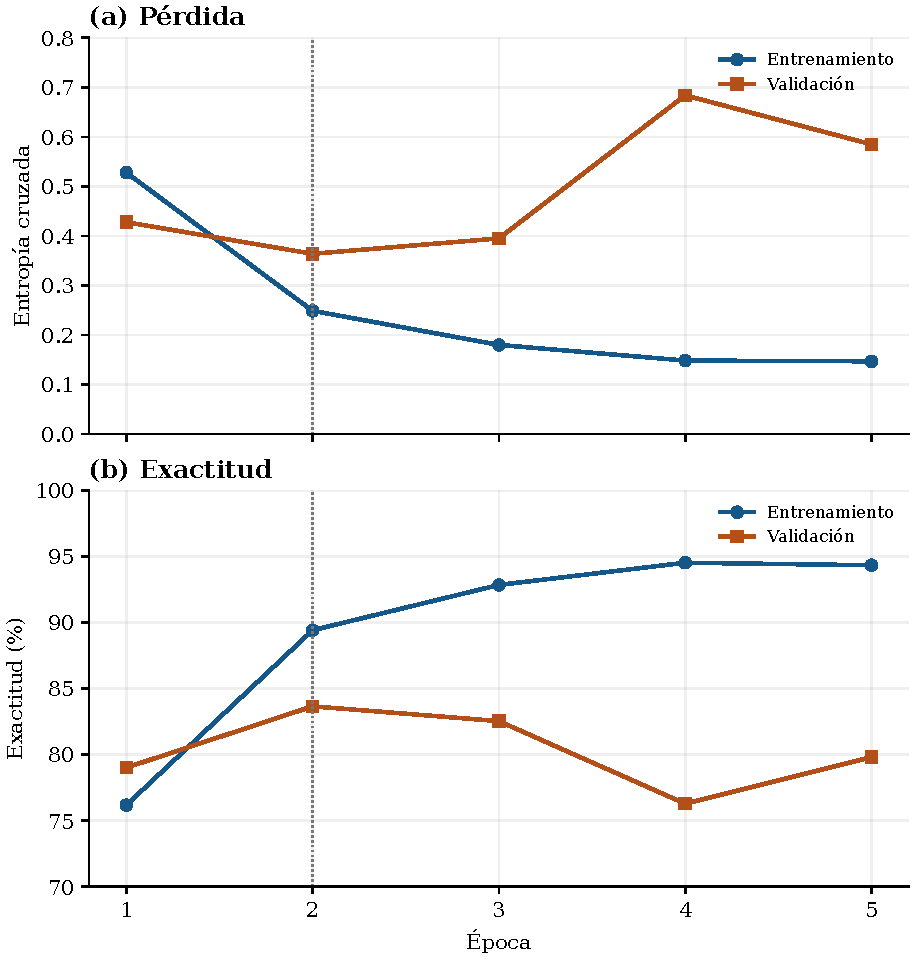
\includegraphics[width=.81\linewidth]{figuras/cap2_curvas_cnn.pdf}
\caption{Evolución de la pérdida y la exactitud registradas durante el entrenamiento de la CNN. La línea vertical identifica la época 2, de menor pérdida y mayor exactitud de validación entre las cinco épocas registradas.}\label{fig:cap2_curvas}
\fuente{elaboración propia a partir de los registros de entrenamiento}
\end{figure}

La menor pérdida de validación, 0,3639, y la mayor exactitud de validación, 83,65\%, se alcanzaron en la segunda época. Al finalizar la quinta época, la pérdida de validación fue 0,5848 y la exactitud, 79,81\%. Por consiguiente, el modelo seleccionado como referencia corresponde al estado final del entrenamiento, cuyo desempeño se distingue del mejor valor intermedio observado.

La reducción de la pérdida de entrenamiento acompañada por el deterioro de la validación a partir de la segunda época es compatible con sobreajuste. Este fenómeno ocurre cuando el modelo se adapta a particularidades de las muestras de entrenamiento que no se traducen en una mejora sobre otras muestras. En la quinta época, los valores registrados de exactitud de entrenamiento y validación presentan una diferencia de 14,52 puntos porcentuales. Este comportamiento motiva evaluar las variantes cuantizadas con un protocolo común, de modo que sus diferencias se interpreten respecto de la misma referencia.

El conjunto de evaluación se utilizó también para supervisar la validación durante el entrenamiento, sin intervenir en el cálculo de los gradientes. En consecuencia, los resultados caracterizan el desempeño sobre el conjunto empleado en el desarrollo y permiten comparar las variantes en condiciones compartidas; su alcance no corresponde a una validación externa independiente.
La campaña QAT posterior registra ocho épocas efectivamente ejecutadas, aunque se había establecido un máximo de quince. El programa informa detención anticipada y restauración de los pesos de la época 4, cuya pérdida de validación interna fue 0,102449. Para este ajuste se utilizaron 2279 imágenes de entrenamiento y 403 de validación interna; la comparación final conserva las 624 imágenes del conjunto de evaluación. Por ello, la exactitud interna de QAT, próxima al 95\%, no se compara directamente con el 79,97\% obtenido sobre el conjunto final.

\resfig{rx_qat.pdf}{Pérdida y exactitud durante las ocho épocas QAT registradas. La línea vertical identifica los pesos restaurados por el procedimiento de detención anticipada.}{fig:res_rx_qat}{\texttt{historial\_\allowbreak qat.csv}}{.96}

La restauración de la mejor época modifica el punto del entrenamiento que se exporta. En consecuencia, las diferencias entre QAT y Float32 incluyen tanto la cuantización como el reajuste de los parámetros. No pueden atribuirse exclusivamente al redondeo de una misma red congelada.

\FloatBarrier
\subsection{Comparación de clasificación y errores por clase}
La evaluación comprende 234 imágenes NORMAL y 390 PNEUMONIA. Las métricas de la Tabla~\ref{tab:xrayres} se verificaron con las etiquetas y predicciones almacenadas para cada variante. Se considera PNEUMONIA como clase positiva. La exactitud balanceada permite observar conjuntamente la sensibilidad y la especificidad, evitando que el mayor número de imágenes de neumonía oculte el comportamiento sobre la clase NORMAL.
\begin{table}[H]
\centering\small
\caption{Desempeño de clasificación sobre 624 radiografías. Valores en porcentaje.}\label{tab:xrayres}
\begin{tabularx}{\linewidth}{Yrrrrr}\toprule
Variante & Exact. & Balanceada & Sensib. & Especif. & $F_1$\\\midrule
Float32 & 79,81 & 73,68 & 98,21 & 49,15 & 85,87\\
PTQ INT8 & 80,93 & 75,34 & 97,69 & 52,99 & 86,49\\
INT16x8 & 79,17 & 72,82 & 98,21 & 47,44 & 85,49\\
Mixed-3 & 79,49 & 73,25 & 98,21 & 48,29 & 85,68\\
Mixed-5 & 79,81 & 73,68 & 98,21 & 49,15 & 85,87\\
QAT INT8 & 79,97 & 74,06 & 97,69 & 50,43 & 85,91\\
\bottomrule\end{tabularx}
\fuente{\texttt{comparacion\_final\_modelos.csv}; comprobación con las predicciones almacenadas}
\end{table}

\resfig{rx_metricas.pdf}{Comparación de exactitud y especificidad en las seis variantes del clasificador.}{fig:res_rx_metricas}{elaboración propia a partir de las métricas verificadas}{1}

PTQ INT8 obtiene 505 clasificaciones correctas de 624, frente a 498 de Float32: la diferencia es de siete imágenes y 1,12 puntos porcentuales. Sin embargo, la sensibilidad se reduce de 98,21\% a 97,69\%, mientras que la especificidad aumenta de 49,15\% a 52,99\%. La mejora de exactitud observada está asociada principalmente a nueve imágenes NORMAL adicionales correctamente clasificadas, a costa de dos neumonías adicionales clasificadas como normales. Este intercambio queda explícito en las matrices de confusión.

\resfig{rx_confusiones.pdf}{Matrices de confusión de los modelos sobre 624 imágenes. Se muestran conteos y porcentajes por fila; las filas representan la clase real.}{fig:res_rx_confusiones}{predicciones y matrices CSV de la evaluación final}{1}

En todas las variantes se observa sensibilidad alta y especificidad considerablemente menor. Por ejemplo, Float32 clasifica correctamente 383 de las 390 neumonías, pero sólo 115 de las 234 imágenes normales. Por tanto, una exactitud cercana al 80\% no describe por sí sola un comportamiento equilibrado entre clases. Estos resultados caracterizan el conjunto utilizado en el desarrollo y no constituyen una validación clínica o externa.

La variante Mixed-5 reproduce las 624 decisiones de Float32. INT16x8 modifica cuatro decisiones y Mixed-3 modifica dos; en ambos casos las modificaciones corresponden a nuevas clasificaciones incorrectas respecto de la referencia. QAT cambia 17 decisiones, corrige nueve errores e introduce ocho, por lo que su mejora neta es de una imagen. La Tabla~\ref{tab:rx_pareadas} muestra el contraste emparejado y evita interpretar dos exactitudes iguales como prueba suficiente de identidad de las predicciones.
\begin{table}[H]
\centering\small
\caption{Cambios de decisión respecto de Float32 sobre las mismas imágenes.}\label{tab:rx_pareadas}
\begin{tabularx}{\linewidth}{Yrrr}\toprule
Variante & Corrige & Introduce error & Decisiones distintas\\\midrule
PTQ INT8 & 25 & 18 & 43\\
INT16x8 & 0 & 4 & 4\\
Mixed-3 & 0 & 2 & 2\\
Mixed-5 & 0 & 0 & 0\\
QAT INT8 & 9 & 8 & 17\\
\bottomrule\end{tabularx}
\fuente{cálculo propio a partir de \texttt{predicciones\_*.npz}}
\end{table}


Aunque PTQ INT8 alcanza la mayor exactitud observada, los resultados de una sola partición y de un único entrenamiento no demuestran que su ventaja sea sistemática. Mixed-5 ofrece una evidencia diferente: conserva las decisiones de la referencia en este conjunto y disminuye el tamaño del archivo. La comparación distingue el desempeño respecto de las etiquetas de la concordancia con Float32.

\FloatBarrier
\subsection{Tamaño, latencia en computador y diferencias de salida}
\begin{table}[H]
\centering\small
\caption{Tamaño y latencia de los modelos evaluados en el computador.}\label{tab:rx_recursos}
\begin{tabularx}{\linewidth}{Yrrrrr}\toprule
Variante & Archivo (B) & Red. (\%) & Media (ms) & P95 (ms) & RMSE salida\\\midrule
Float32 & 95\,652 & 0,00 & 0,173 & 0,276 & 0,000000\\
PTQ INT8 & 38\,824 & 59,41 & 0,531 & 0,913 & 0,519218\\
INT16x8 & 31\,672 & 66,89 & 9,258 & 12,128 & 0,007808\\
Mixed-3 & 31\,968 & 66,58 & 0,299 & 0,408 & 0,005246\\
Mixed-5 & 34\,128 & 64,32 & 0,251 & 0,389 & 0,003778\\
QAT INT8 & 29\,784 & 68,86 & 0,373 & 0,466 & 0,028257\\
\bottomrule\end{tabularx}
\fuente{\texttt{comparacion\_final\_modelos.csv}; reducción respecto de 95\,652 B}
\end{table}

\resfig{rx_recursos_host.pdf}{Tamaño TFLite y latencia media en el computador. La escala temporal es logarítmica para visualizar la diferencia de INT16x8.}{fig:res_rx_host}{\texttt{comparacion\_\allowbreak final\_\allowbreak modelos.csv}}{1}

La referencia utilizada en esta comparación es el archivo Float32 TFLite de 95\,652 B. Con esa base, PTQ INT8 reduce el tamaño en 59,41\%, Mixed-5 en 64,32\% y QAT INT8 en 68,86\%. La comparación utiliza archivos TFLite, de modo que las reducciones se calculan sobre un mismo formato de representación. El menor archivo registrado es QAT INT8, de 29\,784 B.

En el computador, Float32 registra la menor latencia media, 0,173 ms. INT16x8 requiere 9,258 ms, aproximadamente 53,57 veces ese tiempo, mientras que Mixed-5 requiere 0,251 ms. La reducción del número de bits no implica una reducción de latencia en todos los entornos: aquí se observan los tiempos del intérprete y de sus rutas de ejecución en el PC. Estos valores se mantienen separados de los tiempos medidos en la STM32.

El RMSE de las salidas respecto de Float32 es 0,003778 para Mixed-5 y 0,005246 para Mixed-3. PTQ INT8 presenta un RMSE mucho mayor, 0,519218, aun cuando su exactitud de clasificación es ligeramente superior. La comprobación con las matrices de salidas almacenadas reproduce ese valor. Una salida numéricamente diferente puede conservar el orden entre clases y, con ello, la decisión final. Por tanto, el RMSE de las dos salidas y la exactitud responden a preguntas distintas; tampoco debe interpretarse automáticamente cada salida como una probabilidad calibrada.

Existe además una diferencia de topología relevante para la interpretación. Los grafos y registros ST identifican 30\,682 parámetros en PTQ INT8, frente a 22\,700 en INT16x8 y la variante mixta. En el grafo PTQ se observan convoluciones con ocho canales, mientras que la referencia de entrenamiento utiliza seis. Esta evidencia impide tratar toda diferencia entre las variantes desplegadas como efecto aislado de la precisión. Además, las exportaciones PTQ con interfaz Float32 e INT8 se consideran artefactos distintos. Sin una correspondencia explícita de identificadores, topología e interfaz, no se atribuye al archivo desplegado la exactitud obtenida por otro archivo evaluado en PC. Los registros permiten comparar las implementaciones evaluadas, pero no demuestran que todos procedan de una única topología y de los mismos pesos antes de cuantizar.

\FloatBarrier
\section{Clasificación de radiografías: implementación en placa}
\FloatBarrier
\subsection{Fidelidad numérica y tiempo de inferencia}
Los registros de ST Edge AI Core 4.0.1 contienen una validación sobre ocho imágenes, cuatro por clase. El RMSE cruzado de la Tabla~\ref{tab:rx_placa} compara la salida de la implementación ejecutada con la salida del modelo de referencia importado. Un cero informado se limita a las entradas ensayadas y a la resolución del reporte; no acredita identidad matemática para entradas arbitrarias. La exactitud de la última columna compara, en cambio, la clase predicha por la placa con las etiquetas. Las métricas describen, por tanto, propiedades distintas.
\begin{table}[H]
\centering\small
\caption{Validación de radiografías sobre ocho entradas en la STM32N6570-DK.}\label{tab:rx_placa}
\begin{tabularx}{\linewidth}{Yrrrr}\toprule
Variante / ruta & Media (ms) & Mín.--máx. (ms) & RMSE cruzado & Exact. (\%)\\\midrule
INT8 / M55 & 16,621 & 16,580--16,659 & 0 & 75,0\\
INT8 / Neural-ART & 0,514 & 0,506--0,536 & $2,584\times10^{-3}$ & 75,0\\
INT16x8 / M55 & 53,240 & 52,966--53,325 & $3,871\times10^{-5}$ & 62,5\\
INT16x8 / Neural-ART & 0,600 & 0,591--0,627 & $3,171\times10^{-1}$ & 62,5\\
Mixta-5 / M55 & 52,481 & 52,434--52,594 & 0 & 75,0\\
Mixta-5 / Neural-ART & 104,700 & 103,735--104,928 & 0 & 75,0\\
QAT / M55 & 14,814 & 14,805--14,840 & 0 & 75,0\\
QAT / Neural-ART & 0,290 & 0,288--0,305 & $1,092\times10^{-2}$ & 62,5\\
\bottomrule\end{tabularx}
\fuente{registros de validación ST incluidos en el paquete experimental}
\end{table}

\resfig{rx_latencia_placa.pdf}{Latencia media en la STM32N6570-DK para las rutas Cortex-M55 y Neural-ART. La comparación temporal debe leerse junto con la fidelidad numérica de la Tabla~\ref{tab:rx_placa}.}{fig:res_rx_target}{perfiles ST sobre ocho entradas por implementación}{1}

PTQ INT8 registra 16,621 ms en Cortex-M55 y 0,514 ms por la ruta Neural-ART, equivalente a una razón de tiempos de 32,34. La exactitud del pequeño lote es 75\% en ambas rutas; el RMSE cruzado es cero en M55 y 0,002584 en Neural-ART. El resultado documenta una reducción importante de tiempo para esa implementación INT8, con una discrepancia numérica pequeña pero no nula en el acelerador. La exactitud de 75\% corresponde sólo a seis aciertos en ocho entradas y no sustituye a la evaluación de 624 imágenes.

El validador informa RMSE cruzado igual a cero para Mixed-5 en las dos rutas, sobre las entradas ensayadas. Sin embargo, la ruta Neural-ART necesita 104,700 ms, frente a 52,481 ms de Cortex-M55: resulta aproximadamente dos veces más lenta. Por tanto, conservar las salidas del modelo no garantiza aprovechar favorablemente la NPU. La ubicación de las operaciones Float32 y la fragmentación de la ejecución se examinan con el perfil por épocas.

El resultado INT16x8 requiere una interpretación particular. En M55, el reporte de generación indica formato flotante, 90\,800 B de pesos y 533\,652 B de activaciones; el tiempo medido es 53,240 ms. En la ruta Neural-ART, el perfil sí registra actividad hardware y un tiempo de 0,600 ms, pero el RMSE cruzado aumenta a 0,317093. Las salidas de referencia abarcan aproximadamente 0,0146--0,6532, mientras que las de la placa se concentran entre 0,4964 y 0,5049.

Aunque ambas implementaciones de referencia y destino obtienen 62,5\% de exactitud en ese lote Neural-ART, sus matrices de confusión son diferentes: la referencia presenta $(TN,FP,FN,TP)=(1,3,0,4)$ y la placa $(4,0,3,1)$. La igualdad de cinco aciertos sobre ocho imágenes oculta, por tanto, diferencias relevantes en las decisiones. El tiempo de 0,600 ms no se presenta como aceleración equivalente de INT16x8 nativo. La documentación delimita el soporte hardware a operadores y esquemas cuantizados compatibles \cite{cap4_stoperators}; el nombre del archivo de entrada no certifica la precisión realmente ejecutada.


La validación QAT utiliza el mismo hash de modelo en M55 y Neural-ART. M55 registra 14,814 ms, RMSE cruzado informado como cero y seis aciertos sobre ocho imágenes. Neural-ART registra 0,290 ms, RMSE cruzado 0,010918301 y cinco aciertos. Las matrices son $(TN,FP,FN,TP)=(2,2,0,4)$ en referencia/M55 y $(1,3,0,4)$ en NPU: aparece un falso positivo adicional. El cambio de 12,5 puntos porcentuales corresponde a un caso en un lote pequeño, no a una estimación sobre las 624 imágenes de la evaluación en computador.
\resfig{rx_qat_validacion_confusion.pdf}{Validación QAT del clasificador: concordancia de las rutas CPU y diferencia de decisión de la ruta Neural-ART en el lote de ocho imágenes.}{fig:qat_validacion}{matrices de confusión de los registros ST; la comparación incluye la validación L476 descrita al cierre del capítulo}{1}
El perfil QAT de Neural-ART asigna 98,9\% a hardware, 0\% a operadores software y 1,1\% a control software. Es la menor latencia radiográfica registrada, 43,6\% inferior a los 0,514 ms de PTQ INT8, pero no conserva todas las decisiones de referencia del lote. La razón de tiempos entre sus rutas M55 y NPU es 51,08; se trata de una comparación entre implementaciones, no de una medida aislada de una instrucción o unidad.

\FloatBarrier
\subsection{Memoria y transformación de los grafos}
\begin{table}[H]
\centering\small
\caption{Memoria de red informada durante la generación para radiografías.}\label{tab:rx_memoria}
\begin{tabularx}{\linewidth}{Yrr}\toprule
Variante / ruta & Pesos (B) & Activaciones (B)\\\midrule
INT8 / M55 & 30\,832 & 92\,496\\
INT8 / Neural-ART & 30\,689 & 112\,500\\
INT16x8 / M55 & 90\,800 & 533\,652\\
INT16x8 / Neural-ART & 22\,753 & 180\,000\\
Mixta-5 / M55 & 26\,000 & 533\,652\\
Mixta-5 / Neural-ART & 26\,289 & 781\,536\\
QAT / M55 & 22\,828 & 35\,704\\
QAT / Neural-ART & 22\,704 & 55\,368\\
\bottomrule\end{tabularx}
\fuente{primer resumen de \texttt{generate}; incluye búferes de entrada/salida en activaciones}
\end{table}

\resfig{rx_memoria_npu.pdf}{Distribución de memoria de red de todas las variantes radiográficas evaluadas en Neural-ART, incluido QAT.}{fig:rx_memoria_npu}{pesos RO y activaciones RW del primer resumen de generación; 1 KiB = 1024 B}{1}
Las categorías se representan por separado porque los pesos y el espacio de trabajo no equivalen a una única reserva de SRAM. No se incluyen aquí el código, la pila, el heap ni los búferes externos de la aplicación. La figura muestra volumen por categoría, no ubicación física en cada banco. Para QAT/NPU se usan 22\,704 B de pesos y 55\,368 B de activaciones de la generación; los 22\,840 B y 35\,720 B del resumen posterior de validación son diferentes y no se consideran intercambiables sin verificar el alcance de cada campo. Se mantienen las cifras del resumen de generación como base uniforme de esta comparación.
Las cifras de la Tabla~\ref{tab:rx_memoria} se toman del resumen de generación de cada implementación. Esto es especialmente importante en la ruta Neural-ART, porque los resúmenes posteriores pueden informar otros tamaños; la atribución exacta de cada campo a la implementación o a la referencia debe verificarse antes de combinarlos. Para Mixed-5, la generación asigna 781\,536 B a activaciones, mientras que el resumen de validación informa 533\,448 B; utilizar indistintamente ambos valores produciría una comparación inconsistente. El primero concuerda con la distribución de memoria detallada de la implementación generada.

En Mixed-5, la ruta Neural-ART incrementa el búfer de activaciones en 46,45\% respecto de M55. En INT8, el incremento es de 21,63\%. Los pesos de la red y el búfer temporal evolucionan de manera diferente: un menor archivo o menos pesos no implican necesariamente menos memoria de trabajo. Estos tamaños no se presentan como la ocupación completa de Flash o SRAM del firmware.

Las Figuras~\ref{fig:res_rx_original} y~\ref{fig:res_rx_compilado} presentan el grafo importado PTQ INT8 y su representación optimizada. Se conservan los grafos exportados por la herramienta; los diagramas largos se distribuyen en tramos consecutivos para mantener legibles los operadores y las formas de los tensores. El orden de lectura es de arriba abajo en cada tramo y de izquierda a derecha entre tramos; los cortes se sitúan sobre las conexiones para conservar los nodos legibles.
\resfig{rx_int8_original_segmentado.pdf}{Grafo importado del clasificador PTQ INT8, presentado en tres tramos consecutivos. Se observan convoluciones de ocho canales, agrupaciones espaciales, capas densas y conversiones de entrada/salida.}{fig:res_rx_original}{SVG PTQ INT8 previo a la optimización, incluido en los resultados ST}{.97}
\resfig{rx_int8_opt.pdf}{Grafo optimizado de radiografías PTQ INT8 por Neural-ART. Los bloques EC agrupan ejecución coordinada por el controlador de épocas y los bloques SW identifican procesamiento software.}{fig:res_rx_compilado}{SVG PTQ INT8 optimizado exportado por la herramienta}{.70}

La reducción del número de nodos visibles en el grafo compilado no equivale a eliminar las funciones aprendidas: la herramienta reorganiza y agrupa operadores para la ejecución. La interpretación de los bloques debe contrastarse con el perfil temporal y con las salidas validadas. En particular, un bloque EC representa una unidad de planificación de ejecución y no una capa original de la CNN \cite{cap4_stcompiler}.

\resfig{rx_mixed_opt_tramo1.pdf}{Grafo optimizado Neural-ART de radiografías Mixed-5: tramo 1 de 3. La lectura continúa en el tramo siguiente.}{fig:res_rx_mixed_graph}{SVG de la variante selectiva de cinco nodos; recorte consecutivo del grafo completo}{.95}
\resfig{rx_mixed_opt_tramo2.pdf}{Grafo optimizado Neural-ART de radiografías Mixed-5: tramo 2 de 3. La lectura continúa en el tramo siguiente.}{fig:res_rx_mixed_graph2}{SVG de la variante selectiva de cinco nodos; recorte consecutivo del grafo completo}{.95}
\resfig{rx_mixed_opt_tramo3.pdf}{Grafo optimizado Neural-ART de radiografías Mixed-5: tramo 3 de 3. Este tramo completa la secuencia de ejecución.}{fig:res_rx_mixed_graph3}{SVG de la variante selectiva de cinco nodos; recorte consecutivo del grafo completo}{.95}

El perfil de Mixed-5 atribuye 99,6\% del tiempo a software. Dos bloques identificados como convolución Float32 consumen 60,833 y 32,003 ms, respectivamente; juntos representan aproximadamente 88,67\% del tiempo total. En consecuencia, el principal costo observado está en las regiones software de cómputo, no solamente en las conversiones. La asignación de parte de la red a hardware resulta insuficiente para compensar ese costo en la implementación medida.

\FloatBarrier
\subsection{Demostración completa mediante UART}
El registro de transmisión contiene 16 imágenes identificadas por su ruta: ocho NORMAL y ocho PNEUMONIA. Cada respuesta incluye la clase, las dos salidas expresadas en milésimas y la latencia reportada por la aplicación. El archivo y los antecedentes del desarrollo identifican esta demostración como PTQ de precisión mixta selectiva INT8/Float32; el mensaje UART no incorpora por sí mismo una huella del modelo.

Se obtienen 12 aciertos de 16, con cuatro falsos positivos y ningún falso negativo: exactitud de 75\%, sensibilidad de 100\%, especificidad de 50\% y $F_1=80$\%. El primer ejemplo tiene las dos salidas redondeadas a 180 milésimas y la aplicación informa NORMAL; la matriz utiliza la decisión emitida, sin reconstruir otra clase a partir de las cifras redondeadas.
\resfig{rx_uart.pdf}{Matriz de confusión y latencias de la demostración UART con 16 radiografías.}{fig:res_rx_uart}{respuestas \texttt{RESULT} y clase real identificada en las rutas de las imágenes}{1}

La latencia media informada es 105,761 ms, con mínimo de 104,885 ms y máximo de 106,248 ms. Su orden de magnitud es compatible con los 104,700 ms del perfil ST de la variante mixta Neural-ART. Esta proximidad no identifica por sí sola el binario ni permite atribuir la diferencia a un componente específico. La latencia reportada corresponde al intervalo de inferencia definido por la aplicación; el registro no contiene una medición completa del tiempo de transferencia de toda la imagen más inferencia y devolución.

Esta prueba acredita el funcionamiento de la cadena de recepción, inferencia y respuesta para las imágenes enviadas. Su lote reducido y su propósito de integración impiden extrapolar la sensibilidad de 100\% al conjunto de 624 imágenes, donde sí aparecen falsos negativos.

\FloatBarrier
\section{MPC: resultados de simulación y cuantización}
\FloatBarrier
\subsection{Referencia adoptada y fidelidad de la transferencia}\label{sec:equivalencia_mpc}
El desarrollo comprendió una etapa exploratoria de entrenamiento de una red Float32 y un estudio posterior que utiliza el modelo de referencia de los autores, transferido de Equinox a Keras. Se toma este último como base de la comparación de cuantizaciones, porque contiene la evaluación común de 200 condiciones iniciales y la exportación de las variantes posteriormente validadas. Las conclusiones de la etapa exploratoria no se mezclan con las cifras de esa campaña.

En la etapa exploratoria, la reproducción de trayectorias con las acciones del conjunto de datos ya presentaba diferencias antes de atribuirlas a una red cuantizada. El resumen sobre diez trayectorias informa RMSE medios de posición de 0,018836 m y de ángulo de 1,973763 rad. Este antecedente delimita el alcance de aquella comparación MPC--red: una discrepancia en la reproducción de la planta impide interpretar todo error de trayectoria como error de aproximación neuronal. La evaluación final emplea la referencia y el procedimiento descritos en Metodología.
El procedimiento de comparación se describe en la sección~\ref{sec:comparacion_transferencia}.

\begin{table}[H]\centering\small
\caption{Error EQX--Keras registrado sobre las entradas comunes.}\label{tab:cap2_equivalencia}
\begin{tabularx}{\linewidth}{lYY}\toprule
Métrica & Salida normalizada & Desnormalizada y saturada (V)\\\midrule
RMSE & $9{,}1202736\times10^{-7}$ & $8{,}20341354601202\times10^{-6}$\\
MAE & $2{,}58891\times10^{-7}$ & $2{,}3063083409957656\times10^{-6}$\\
Máximo absoluto & $4{,}0628016\times10^{-5}$ & $3{,}6565214761175024\times10^{-4}$\\\bottomrule
\end{tabularx}
\fuente{evaluación numérica de la transferencia EQX--Keras}
\end{table}
El RMSE físico equivale aproximadamente a 8,20 $\mu$V y el error máximo a 0,366 mV en las muestras comparadas. La transferencia conserva con alta fidelidad la salida de la red cargada. No obstante, el error no es nulo: igualdad de parámetros transferidos no implica identidad bit a bit de las operaciones entre entornos. Las diferencias son compatibles con distintas evaluaciones numéricas de productos y activaciones, sin que esta prueba aislada permita atribuir una causa única.





\begin{table}[H]\centering\small
\caption{Comparación emparejada de resultados en lazo cerrado.}\label{tab:cap2_pareado}
\begin{tabularx}{\linewidth}{Yr}\toprule
Resultado & Número de condiciones\\\midrule
Éxito en ambos modelos & 193\\
Éxito sólo en EQX & 1\\
Éxito sólo en Keras & 6\\
Fallo en ambos modelos & 0\\\midrule
Total & 200\\\bottomrule
\end{tabularx}
\fuente{evaluación de los controladores EQX y Keras sobre 200 condiciones iniciales}
\end{table}
Se obtuvieron 194 éxitos EQX (97\%) y 199 éxitos Keras (99,5\%), con siete condiciones de resultado distinto. El promedio de RMSE de acción por trayectoria fue de 0,8067067 V y la diferencia máxima global de acción alcanzó 9,5751839 V. Estas cifras corresponden a trayectorias que evolucionan por separado, no a la comparación de acciones ante un mismo estado.

En lazo cerrado, diferencias pequeñas pueden modificar los estados posteriores y amplificarse en trayectorias sensibles o cercanas al límite de un criterio de éxito. La influencia de la precisión aritmética y del procedimiento de integración impide atribuir esas diferencias a una causa única a partir de esta comparación. Los resultados distinguen, por tanto, la alta fidelidad de la transferencia sobre entradas comunes de la equivalencia de trayectorias. La referencia Keras alcanzó una tasa de éxito de 99,5\% en el banco de prueba definido.
\FloatBarrier
\subsection{Resultado de las variantes en 200 condiciones iniciales}
\begin{table}[H]
\centering\small
\caption{Resultados en lazo cerrado sobre 200 condiciones iniciales.}\label{tab:mpcres}
\begin{tabularx}{\linewidth}{Yrrrrl}\toprule
Variante & Éxitos & Fallos & Éxito (\%) & Archivo (B) & Formato\\\midrule
Float32 Keras & 199 & 1 & 99,5 & 97\,905 & .keras\\
PTQ INT8 tensor & 74 & 126 & 37,0 & 22\,440 & .tflite\\
PTQ INT8 canal & 50 & 150 & 25,0 & 30\,672 & .tflite\\
QAT INT8 & 65 & 135 & 32,5 & 23\,568 & .tflite\\
PTQ INT16x8 & 198 & 2 & 99,0 & 35\,624 & .tflite\\
Mixta selectiva & 156 & 44 & 78,0 & 55\,360 & .tflite\\
\bottomrule\end{tabularx}
\fuente{exportación HTML del estudio MPC de referencia; el conteo Keras procede de su evaluación explícita}
\end{table}

\resfig{mpc_exito.pdf}{Tasa de éxito en lazo cerrado para las seis variantes del controlador. Todas las tasas se refieren a 200 condiciones iniciales del banco de simulación.}{fig:res_mpc_exito}{resultados de la exportación HTML del estudio MPC de referencia}{1}

La referencia Keras alcanza 199 éxitos de 200. PTQ INT8 por tensor reduce el resultado a 74 éxitos; PTQ por canal, a 50; y QAT INT8, a 65. El ajuste QAT no recupera el nivel Float32 y tampoco supera al PTQ por tensor en esta campaña. El esquema por canal, pese a ofrecer escalas diferenciadas para los pesos, no obtiene una ventaja funcional en el banco evaluado. No se deduce de ello una inferioridad general del método: el resultado depende de esta red, de su conversión y del criterio de control.

INT16x8 conserva 198 éxitos, a sólo un caso de la referencia. La precisión mixta recupera 156 éxitos, es decir, 41 puntos porcentuales más que PTQ por tensor, pero permanece 21,5 puntos por debajo de Keras. De esta comparación se infiere que preservar mayor precisión en determinadas regiones o activaciones es relevante para este controlador. Los resultados no aíslan una causa única ni constituyen una demostración formal de estabilidad.

Los tamaños consignados en la Tabla~\ref{tab:mpcres} requieren distinguir el formato: 97\,905 B corresponde al archivo \texttt{.keras} de referencia, mientras que los restantes son archivos \texttt{.tflite}. Por ello no se utiliza esa fila para calcular un porcentaje de compresión atribuible exclusivamente al ancho de los datos. Entre archivos TFLite cuantizados, INT16x8 ocupa 35\,624 B y la variante mixta 55\,360 B. Su ventaja funcional no coincide con el mínimo tamaño, que corresponde al PTQ por tensor de 22\,440 B.

Las Figuras~\ref{fig:res_mpc_tray1} a~\ref{fig:res_mpc_control2} reproducen las curvas almacenadas para una condición de demostración común. Se presentan posición, ángulo y acción de control para visualizar la recuperación angular, las oscilaciones y las saturaciones, sin sustituir el resultado agregado de las 200 condiciones. Las señales de control se muestran con retención entre instantes de muestreo.
\resfig{mpc_tray_1_pos.pdf}{Posición del carro en simulación: Float32 Keras, PTQ INT8 por tensor y PTQ INT8 por canal, de arriba abajo. Curvas de la condición de demostración.}{fig:res_mpc_tray1}{figuras de la exportación HTML del estudio MPC final}{1}
\resfig{mpc_tray_1_angulo.pdf}{Ángulo del péndulo en simulación: Float32 Keras, PTQ INT8 por tensor y PTQ INT8 por canal, de arriba abajo. Se conservan la banda final de $\pm0{,}17$ rad y el inicio de las diez últimas muestras de los gráficos originales.}{fig:res_mpc_angulo1}{figuras originales de la exportación HTML del estudio MPC final}{1}
\resfig{mpc_tray_1_u.pdf}{Acción de control en simulación: Float32 Keras, PTQ INT8 por tensor y PTQ INT8 por canal, de arriba abajo. Se conserva la representación discreta original.}{fig:res_mpc_control1}{figuras de la exportación HTML del estudio MPC final}{1}
\resfig{mpc_tray_2_pos.pdf}{Posición del carro en simulación: QAT INT8, INT16x8 y precisión mixta, de arriba abajo. Curvas de la condición de demostración.}{fig:res_mpc_tray2}{figuras de la exportación HTML del estudio MPC final}{1}
\resfig{mpc_tray_2_angulo.pdf}{Ángulo del péndulo en simulación: QAT INT8, INT16x8 y precisión mixta, de arriba abajo. Se conservan la banda final de $\pm0{,}17$ rad y el inicio de las diez últimas muestras de los gráficos originales.}{fig:res_mpc_angulo2}{figuras originales de la exportación HTML del estudio MPC final}{1}
\resfig{mpc_tray_2_u.pdf}{Acción de control en simulación: QAT INT8, INT16x8 y precisión mixta, de arriba abajo. Se conserva la representación discreta original.}{fig:res_mpc_control2}{figuras de la exportación HTML del estudio MPC final}{1}

Los gráficos angulares muestran una pérdida tardía de recuperación en el ejemplo PTQ por tensor, mientras que la referencia Float32 y el ejemplo INT16x8 se mantienen próximos al equilibrio tras el transitorio. La trayectoria particular de QAT y la de PTQ por canal deben interpretarse junto con su baja tasa agregada: una condición favorable no representa el conjunto de 200 ensayos.

Las curvas INT8 muestran actividad de control persistente y mayor oscilación de posición que la referencia y el ejemplo INT16x8. La variante mixta mejora el cumplimiento final en la condición ilustrada, pero conserva transitorios relevantes. Un ejemplo favorable de PTQ por canal tampoco contradice su tasa agregada de 25\%: cumplir en una condición particular y hacerlo en todo un banco son propiedades distintas.

\FloatBarrier
\subsection{Diagnóstico de cuantización y precisión mixta obtenida}
La auditoría del grafo TFLite de la variante mixta registra 11 operadores Float32, cuatro INT8 y cuatro conversiones. Las capas densas 0, 2, 3, 4, 5 y la salida permanecen en Float32; las capas densas 1 y 6 se ejecutan en INT8 dentro de la representación exportada. Esta composición está documentada en la inspección de tipos, por lo que la denominación de precisión mixta se sustenta en el grafo y no sólo en una opción solicitada al convertidor.
\resfig{mpc_sensibilidad.pdf}{Diagnóstico de error normalizado por escala utilizado en la selección de capas del MPC mixto. Las capas inicial y de salida se preservaron adicionalmente por decisión del procedimiento.}{fig:res_mpc_sensibilidad}{tabla de sensibilidad por capa de la exportación HTML del estudio MPC}{1}

Los mayores valores del indicador corresponden a las capas densas 3, 4, 2 y 5. La combinación del umbral 0,32 con la conservación explícita de entrada y salida explica qué capas fueron solicitadas en Float32. El resultado de 78\% demuestra una recuperación parcial bajo esta selección, pero no demuestra que el umbral o el conjunto de capas sea óptimo, pues no se realizó una búsqueda exhaustiva de las asignaciones posibles.

\FloatBarrier
\section{MPC: validación y perfil en la STM32N6570-DK}
\FloatBarrier
\subsection{Concordancia numérica y latencia}
\begin{table}[H]
\centering\small
\caption{Validación de MPC sobre 200 entradas en la STM32N6570-DK.}\label{tab:mpc_placa}
\begin{tabularx}{\linewidth}{Yrrr}\toprule
Variante / ruta & Media (ms) & Mín.--máx. (ms) & RMSE cruzado\\\midrule
Float32 / M55 & 0,303 & 0,277--0,316 & $1,298\times10^{-6}$\\
INT8 tensor / M55 & 0,128 & 0,115--0,164 & 0\\
INT8 tensor / NPU & 0,067 & 0,067--0,085 & $1,434\times10^{-2}$\\
INT8 canal / M55 & 0,237 & 0,227--0,364 & 0\\
INT8 canal / NPU & 0,067 & 0,067--0,085 & $2,375\times10^{-2}$\\
QAT / M55 & 0,136 & 0,128--0,176 & 0\\
QAT / NPU & 0,067 & 0,067--0,086 & $1,351\times10^{-2}$\\
INT16x8 / M55 & 0,303 & 0,273--0,315 & $8,705\times10^{-4}$\\
Mixta / M55 & 0,326 & 0,315--0,338 & $4,700\times10^{-8}$\\
Mixta / NPU & 0,480 & 0,467--0,493 & $2,172\times10^{-3}$\\
\bottomrule\end{tabularx}
\fuente{registros de validación ST incluidos en el paquete experimental}
\end{table}

\resfig{mpc_latencia_placa.pdf}{Tiempo medio del controlador por ruta de implementación. La evaluación corresponde a 200 inferencias aisladas, no a 200 simulaciones HIL.}{fig:res_mpc_target}{perfiles ST del caso MPC}{1}

En Cortex-M55, Float32 requiere 0,303 ms. PTQ INT8 por tensor necesita 0,128 ms; QAT INT8, 0,136 ms; y PTQ por canal, 0,237 ms. Sus RMSE cruzados aparecen como cero con la precisión de impresión del reporte. La fidelidad respecto de cada modelo cuantizado no corrige la pérdida de desempeño que ese mismo modelo ya presenta en simulación: una implementación puede reproducir correctamente una política cuyo éxito en lazo cerrado es bajo.

Las tres variantes INT8 por Neural-ART registran 0,067 ms. Las razones de tiempo respecto de sus implementaciones M55 son aproximadamente 1,91 para PTQ por tensor, 3,54 para PTQ por canal y 2,03 para QAT. Sin embargo, sus RMSE cruzados son 0,014340, 0,023751 y 0,013510, respectivamente, superiores a los consignados en las rutas M55. Estas cifras se refieren a la salida normalizada de la red, no directamente a voltios ni a error de trayectoria. No se dispone de HIL para cada una de esas implementaciones NPU que permita cuantificar su efecto acumulado en el control.

La variante mixta requiere 0,326 ms en M55 y 0,480 ms en Neural-ART. M55 presenta RMSE cruzado de $4{,}7\times10^{-8}$, frente a 0,002172 de Neural-ART. En este caso, la ruta M55 resulta 1,47 veces más rápida y conserva mayor concordancia numérica con el modelo importado en las entradas evaluadas. Este resultado sustenta su uso en el banco HIL de la alternativa mixta, sin demostrar por sí solo su superioridad frente a todas las alternativas de control.

\FloatBarrier
\subsection{Resultado de compilación de INT16x8 y memoria de red}
\begin{table}[H]
\centering\small
\caption{Memoria de red informada durante la generación para MPC.}\label{tab:mpc_memoria}
\begin{tabularx}{\linewidth}{Yrr}\toprule
Variante / ruta & Pesos (B) & Activaciones (B)\\\midrule
Float32 / M55 & 62\,404 & 400\\
INT8 tensor / M55 & 16\,656 & 304\\
INT8 tensor / NPU & 15\,331 & 130\\
INT8 canal / M55 & 16\,656 & 704\\
INT8 canal / NPU & 15\,331 & 130\\
QAT / M55 & 16\,656 & 304\\
QAT / NPU & 15\,331 & 130\\
INT16x8 / M55 & 62\,404 & 400\\
Mixta / M55 & 47\,404 & 852\\
Mixta / NPU & 47\,201 & 616\\
\bottomrule\end{tabularx}
\fuente{primer resumen de \texttt{generate}; incluye búferes de entrada/salida en activaciones}
\end{table}

\resfig{mpc_memoria_npu.pdf}{Distribución de memoria de red de las cuatro variantes MPC evaluadas en Neural-ART. Los paneles mantienen escalas independientes para pesos y activaciones.}{fig:mpc_memoria_npu}{primer resumen de generación ST de cada variante}{1}
Las tres variantes INT8 NPU coinciden en 15\,331 B de pesos y 130 B de activaciones; la mixta utiliza 47\,201 B y 616 B. Esta distribución corresponde a la memoria reportada de la red y no a la ocupación total de Flash o SRAM del firmware.
El modelo INT16x8 del MPC se importa como formato flotante en la ruta M55. El reporte indica 62\,404 B de pesos, 400 B de activaciones y 0,303 ms de inferencia, iguales a las magnitudes principales de la implementación Float32. La inspección del código compilado es coherente con cálculo flotante. Por tanto, el 99\% de éxito del archivo INT16x8 en simulación no equivale a disponer de una implementación INT16x8 nativa con ese mismo costo en el microcontrolador.

El RMSE cruzado de esta conversión es 0,000871 en las 200 entradas. La diferencia es pequeña en esa prueba puntual, pero el resultado funcional de la implementación convertida no se ha medido con las 200 condiciones en lazo cerrado. Se conserva así la distinción entre el formato de origen, el resultado de compilación y la tasa de éxito del controlador exportado.

Para las variantes INT8, la generación Neural-ART informa 15\,331 B de pesos y 130 B de activaciones. La variante mixta necesita 47\,201 B y 616 B, respectivamente. En M55, los pesos mixtos ocupan 47\,404 B, una reducción de 24,04\% frente a los 62\,404 B de Float32; el búfer de activaciones aumenta de 400 a 852 B. Preservar regiones Float32 reduce el ahorro de pesos y puede aumentar la memoria temporal, aunque recupere parte del comportamiento de control.

\FloatBarrier
\subsection{Del grafo TFLite al programa de épocas}
\resfig{mpc_mixed_original_segmentado.pdf}{Grafo importado del controlador de precisión mixta. Las conversiones delimitan regiones enteras y flotantes; el diagrama se presenta en tres tramos consecutivos.}{fig:res_mpc_original}{SVG del modelo mixto antes de la optimización}{.76}
\resfig{mpc_mixed_opt_tramo1.pdf}{Grafo optimizado Neural-ART de MPC mixto: tramo 1 de 3. La lectura continúa en el tramo siguiente.}{fig:res_mpc_compilado}{SVG optimizado del MPC mixto; recorte consecutivo del grafo completo}{.95}
\resfig{mpc_mixed_opt_tramo2.pdf}{Grafo optimizado Neural-ART de MPC mixto: tramo 2 de 3. La lectura continúa en el tramo siguiente.}{fig:res_mpc_compilado2}{SVG optimizado del MPC mixto; recorte consecutivo del grafo completo}{.95}
\resfig{mpc_mixed_opt_tramo3.pdf}{Grafo optimizado Neural-ART de MPC mixto: tramo 3 de 3. Este tramo completa la secuencia de ejecución.}{fig:res_mpc_compilado3}{SVG optimizado del MPC mixto; recorte consecutivo del grafo completo}{.95}

El reporte de generación del MPC mixto cuenta 23 épocas computacionales: 21 software y dos hardware. También informa 14 bloques del controlador de épocas, mientras que el perfil presenta 35 bloques ejecutados. Estos conteos pertenecen a niveles diferentes de representación y planificación; no se utilizan como cantidades intercambiables ni como porcentajes de cómputo acelerado. En el detalle software aparecen convoluciones Float32, sumas, tangentes hiperbólicas y conversiones. El uso de una rutina denominada convolución no modifica la descripción de la red original como MLP: corresponde a su representación de implementación.

\resfig{mpc_int8_opt.pdf}{Grafo optimizado del MPC PTQ INT8 por tensor. La agrupación en un bloque EC visible contrasta con la fragmentación del modelo mixto.}{fig:res_mpc_int8graph}{SVG optimizado de PTQ INT8 por tensor}{.95}

La Figura~\ref{fig:res_mpc_int8graph} muestra que una representación compacta de ejecución puede agrupar varias capas de la red. El perfil INT8 asigna 98,7\% del tiempo a hardware. En el modelo mixto, en cambio, la fracción hardware es 9,5\%, con 84,1\% de software y 6,4\% de control software. Esta distribución es consistente con la ausencia de aceleración neta observada para la variante mixta.

\FloatBarrier
\section{MPC: evaluación HIL de la alternativa mixta}
\FloatBarrier
\subsection{Comprobación de las trayectorias y del criterio final}
La campaña HIL comprende los ángulos iniciales $\alpha_0=\pm0{,}10$, $\pm0{,}30$, $\pm1{,}00$ y $\pm3{,}13$ rad, con posición y velocidades iniciales nulas. Cada ensayo contiene 100 acciones separadas por un paso de simulación de 0,16 s. La placa ejecuta la política y el computador integra la planta; por tanto, la evidencia corresponde a un controlador físico conectado a una planta simulada.

Los CSV almacenan el estado previo a cada acción, desde $t=0$ hasta $t=15{,}84$ s. El programa evalúa, en cambio, una secuencia de 101 estados que incluye $t=16$ s. Para reproducir exactamente su ventana final se reconstruyó el último estado mediante el integrador y los parámetros del programa de simulación, aplicando la última acción registrada. La comprobación de los otros 99 pasos contra el CSV dio una diferencia máxima inferior a $5\times10^{-13}$ en las componentes numéricas. El estado de 16 s es un cálculo derivado, no una nueva muestra recibida por UART.

La ventana final corresponde a diez estados entre 14,56 y 16,00 s. Se verifican las restricciones $|y|<0{,}4$ m en toda la trayectoria y $|u|\leq9$ V en las acciones, junto con $|y|<0{,}1$ m y $|e_\alpha|<0{,}17$ rad en la ventana final. La Tabla~\ref{tab:hilres} coincide con los indicadores de éxito de los ocho registros de consola.
\begin{table}[H]
\centering\small
\caption{Verificación funcional de las ocho condiciones iniciales HIL.}\label{tab:hilres}
\begin{tabularx}{\linewidth}{Yrrrrl}\toprule
$\alpha_0$ (rad) & $\max |y|$ (m) & $\max |u|$ (V) & $\max_{10}|y|$ (m) & $\max_{10}|e_\alpha|$ (rad) & Cumple\\\midrule
-3,13 & 0,3588 & 9,000 & 0,1536 & 0,0359 & No\\
-1,00 & 0,1968 & 9,000 & 0,0731 & 0,0368 & Sí\\
-0,30 & 0,2110 & 9,000 & 0,1313 & 2,7736 & No\\
-0,10 & 0,1944 & 9,000 & 0,1475 & 0,0989 & No\\
0,10 & 0,1208 & 5,320 & 0,0278 & 0,0260 & Sí\\
0,30 & 0,1700 & 8,434 & 0,0828 & 0,0250 & Sí\\
1,00 & 0,2079 & 8,836 & 0,0547 & 0,0693 & Sí\\
3,13 & 0,3595 & 9,000 & 0,0954 & 0,0531 & Sí\\
\bottomrule\end{tabularx}
\fuente{CSV HIL; ventana final de 14,56 a 16,00 s, con estado terminal reconstruido}
\end{table}


Cinco ensayos cumplen el criterio final: $+0{,}10$, $+0{,}30$, $+1{,}00$, $-1{,}00$ y $+3{,}13$ rad. Los tres restantes no lo cumplen, aunque todos respetan la restricción global de posición y la saturación de control. El resultado de cinco sobre ocho equivale a 62,5\% en esta selección, pero no se interpreta como estimación de la tasa de éxito sobre todo el espacio de estados ni se compara directamente con el 78\% de las 200 condiciones simuladas.

\resfig{hil_posiciones.pdf}{Posición en los ocho ensayos HIL. Líneas punteadas: restricción global de $\pm0{,}4$ m; líneas discontinuas: banda final de $\pm0{,}1$ m. La zona sombreada identifica la ventana final evaluada.}{fig:res_hil_pos}{CSV HIL y reconstrucción del estado de 16 s}{.96}
\resfig{hil_angulos.pdf}{Error angular equivalente en los ocho ensayos HIL y banda final de $\pm0{,}17$ rad. El criterio se aplica a toda la ventana sombreada, no sólo a la última muestra.}{fig:res_hil_ang}{CSV HIL y reconstrucción del estado de 16 s}{.96}

En $\alpha_0=-0{,}10$ rad, el error angular final permanece dentro de la banda, pero la posición alcanza 0,1475 m en valor absoluto durante la ventana, por encima del límite de 0,1 m. En $\alpha_0=-3{,}13$ rad ocurre una situación semejante: el error angular máximo final es sólo 0,0359 rad, mientras que la posición alcanza 0,1536 m. Un ángulo próximo al equilibrio no basta para declarar éxito.

En $\alpha_0=-0{,}30$ rad, la ventana final contiene un error angular máximo de 2,7736 rad y una posición absoluta máxima de 0,1313 m. Aunque el ángulo en el último instante vuelve a estar próximo al equilibrio, la trayectoria no satisface la condición durante las diez muestras. Este ensayo evidencia la diferencia entre una recuperación instantánea al terminar y el cumplimiento sostenido dentro de la ventana establecida.

\FloatBarrier
\subsection{Representación angular, transitorios y acción de control}
El programa HIL transmite el ángulo continuo en el paquete UART. El ajuste angular se utiliza para calcular el error equivalente y evaluar la orientación del péndulo. Esta inspección elimina la hipótesis de un envolvimiento adicional en el transmisor Python de esta versión. Los CSV no contienen la entrada interna del modelo en C ni una huella del ejecutable cargado; por ello no permiten verificar por sí solos todo el preprocesamiento del firmware. No se atribuyen los fallos observados a una doble normalización sin evidencia.

\resfig{hil_detalles.pdf}{Detalle de los ensayos HIL $\alpha_0=+3{,}13$ y $-0{,}30$ rad. Se distinguen ángulo continuo y error equivalente, posición del carro y acción de control retenida entre muestras.}{fig:res_hil_detalle}{CSV HIL; último estado reconstruido con la planta del programa}{1}

Para $+3{,}13$ rad se observa una recuperación final después de un transitorio que incluye una rotación. El cumplimiento del criterio final no implica permanencia continua cerca del equilibrio desde el primer acercamiento. Asimismo, los ángulos finales próximos a múltiplos de $2\pi$ representan orientaciones equivalentes, pero no describen trayectorias idénticas ni garantizan igual respuesta de una política que recibe el ángulo continuo.

Las diferencias entre ángulos iniciales de signos opuestos muestran que esta campaña no presenta una simetría funcional completa. Los ocho ensayos no permiten identificar una causa única: cuantización, política aproximada, representación de estados y dinámica pueden intervenir. Se conserva la observación empírica sin convertirla en una explicación causal no comprobada.

\FloatBarrier
\subsection{Tiempos de inferencia, comunicación y ejecución del computador}
\begin{table}[H]
\centering\small
\caption{Resumen temporal por condición inicial HIL: 100 intercambios por ensayo.}\label{tab:hil_tiempos}
\begin{tabularx}{\linewidth}{Yrrrr}\toprule
$\alpha_0$ (rad) & Infer. media ($\mu$s) & Infer. máx. ($\mu$s) & RTT medio (ms) & RTT máx. (ms)\\\midrule
-3,13 & 337,55 & 347 & 5,0901 & 5,3027\\
-1,00 & 337,42 & 348 & 5,0928 & 5,2870\\
-0,30 & 337,19 & 353 & 5,0863 & 5,3675\\
-0,10 & 337,25 & 345 & 5,0708 & 5,1602\\
0,10 & 336,99 & 348 & 5,0780 & 5,2427\\
0,30 & 336,76 & 350 & 5,0849 & 5,2873\\
1,00 & 337,17 & 347 & 5,0794 & 5,2479\\
3,13 & 337,44 & 347 & 5,0994 & 5,2156\\
\bottomrule\end{tabularx}
\fuente{cálculo propio a partir de las 800 filas de los CSV HIL}
\end{table}

\resfig{hil_tiempos.pdf}{Distribución de la inferencia y del tiempo de ida y vuelta UART en los ocho ensayos HIL. Cada distribución contiene 100 intercambios.}{fig:res_hil_tiempos}{800 registros temporales de los CSV HIL}{1}

En los 800 intercambios no se registra un RTT superior al período nominal de 160 ms. El mayor tiempo de inferencia observado es 353 $\mu$s y el mayor RTT es 5,3675 ms, aproximadamente 3,35\% de ese período. Estos valores muestran margen temporal en la inferencia y en el intercambio medidos, dentro de las condiciones del ensayo. No constituyen una cota de peor caso garantizada para cualquier carga de ejecución.

Los registros de consola de siete ensayos informan, además, 100 ciclos tardíos del PC, incluyendo el procesamiento del gráfico. El archivo de $+0{,}10$ rad omite esa línea, por lo que no se le asigna un conteo. El tiempo simulado avanza con pasos fijos de 0,16 s, aunque el programa del computador pueda atrasarse respecto del reloj de pared. En consecuencia, cero incumplimientos UART no acredita que todo el banco se haya ejecutado en tiempo real estricto. El resultado funcional describe la planta discretizada con el paso previsto y las acciones de la placa; la sincronización integral del PC constituye una medición distinta.

La inferencia media HIL se sitúa entre 336,76 y 337,55 $\mu$s por ensayo, algo por encima de los 326 $\mu$s del perfil ST de la variante mixta M55. Ambos registros pertenecen a contextos de ejecución diferentes, por lo que no se atribuye automáticamente la diferencia al transporte UART ni a una operación concreta. El RTT, próximo a 5,08 ms, incluye el intercambio completo definido por el script y es considerablemente mayor que la inferencia aislada.

\FloatBarrier
\section{Síntesis de la evidencia de implementación}
La inspección estática de 23 listados complementa los informes de compilación y los perfiles temporales. En los núcleos cuantizados identificados del Cortex-M55 se observaron instrucciones MVE; en los seis listados Cortex-M4 no se encontraron y cinco contienen instrucciones DSP. Los ejecutables orientados a Neural-ART incluyen el código del procesador anfitrión, por lo que sus instrucciones no representan la aritmética interna de la NPU.

\begin{table}[htbp]
\centering\small
\caption{Síntesis de la evidencia estática de las implementaciones.}
\begin{tabular}{p{0.22\linewidth}p{0.67\linewidth}}
\hline
Ruta & Evidencia observada \\\hline
Cortex-M55 & Instrucciones MVE en los núcleos cuantizados identificados; también existen regiones escalares. \\
Cortex-M4 & Sin MVE en los seis listados; instrucciones DSP en cinco y cálculo flotante escalar en la variante MPC importada como INT16x8. \\
Neural-ART & El listado describe el anfitrión; la asignación a NPU se establece con los informes de compilación y los perfiles. \\\hline
\end{tabular}
\end{table}

Esta evidencia identifica recursos presentes en el código, sin cuantificar su contribución temporal. La comparación de despliegue se fundamenta en las latencias, la memoria, la concordancia de salida y la validación funcional presentadas en este capítulo. Las tablas detalladas, los extractos y sus límites de interpretación se conservan en el Anexo~\ref{anexo:instrucciones}.

\section{Síntesis de los resultados por aplicación}\label{sec:sintesis_resultados}
\begin{table}[htbp]\centering\small
\caption{Resultados principales y alcance de la evidencia para la selección por aplicación.}\label{tab:res_sintesis}
\begin{tabularx}{\linewidth}{p{2.5cm}YY}\toprule
Caso & Resultado observado & Implicación sustentada\\\midrule
Radiografías & PTQ INT8: 80,93\% en PC; 0,514 ms en Neural-ART & Alternativa rápida en los registros, con diferencia de topología que limita atribuir todo el beneficio a cuantización\\
Radiografías & QAT: 0,290 ms en Neural-ART; 5/8 aciertos frente a 6/8 de referencia & Menor tiempo observado con una decisión adicional incorrecta en el lote validado\\
Radiografías & Mixed-5 conserva las 624 decisiones Float32; 104,700 ms en Neural-ART & Fidelidad de clasificación sin ventaja temporal de esa ruta frente a M55\\
MPC & INT16x8: 198/200 éxitos; compilación M55 flotante & Alto desempeño del archivo en simulación; no evidencia ejecución INT16x8 nativa\\
MPC & INT8: 0,067 ms en Neural-ART y 25--37\% de éxito en PC & Latencia favorable y desempeño funcional insuficiente respecto de la referencia evaluada\\
MPC & Mixta: 156/200 éxitos en PC; 5/8 en HIL & Recuperación parcial y funcionamiento del banco, con fallos de criterio final identificados\\\bottomrule
\end{tabularx}
\fuente{síntesis de las tablas y figuras de este capítulo}
\end{table}

La selección depende de la aplicación. En radiografías, varias alternativas conservan decisiones similares y presentan costos de implementación muy diferentes. En MPC, la cuantización modifica de forma más pronunciada el cumplimiento del criterio de lazo cerrado, aun cuando la placa reproduzca fielmente el archivo cuantizado.

La precisión mixta recupera parte del comportamiento de referencia, pero no es automáticamente la alternativa más rápida ni la de menor memoria. Los ensayos HIL confirman su operación integrada e identifican tres incumplimientos del criterio final. Estos resultados sustentan la discusión posterior, manteniendo diferenciadas la simulación, la inferencia en placa y la evaluación funcional del control.

\FloatBarrier
\section{Comparación final entre STM32N6570-DK y NUCLEO-L476RG}\label{sec:comparacion_placas}
\subsection{Cobertura, configuración y concordancia de modelos}
La campaña complementaria añade seis validaciones satisfactorias en NUCLEO-L476RG: cinco variantes del MPC sobre 200 entradas cada una y QAT de radiografías sobre ocho imágenes. La campaña no incluye un registro de validación independiente de MPC Float32 en esa placa. Los registros identifican el mismo \texttt{model\_\allowbreak hash} de origen que las variantes correspondientes en STM32N6, y nombran los conjuntos de entrada del procedimiento previo. Esta coincidencia respalda el emparejamiento por modelo; no sustituye una huella del firmware activo o de todos los archivos de entrada. La ejecución NPU, además, informa que omite la comprobación de firma de la red C.

Los perfiles registran CPU a 80 MHz en L476 y a 800 MHz en N657; la ruta Neural-ART informa NPU a 1000 MHz. El STM32L476RG dispone de Cortex-M4, FPU, extensión DSP, 1 MB de Flash y hasta 128 KB de SRAM \cite{res_stl476}. Los registros L476 indican prelectura y cachés del acelerador ART de acceso a Flash; esta unidad no es la NPU Neural-ART. Las diferencias de arquitectura, frecuencia, jerarquía de memoria y bibliotecas impiden interpretar el cociente temporal entre placas como un efecto exclusivo de Helium.
\begin{table}[H]
\centering\small
\caption{Validación aislada en la NUCLEO-L476RG.}\label{tab:nucleo_validacion}
\begin{tabularx}{\linewidth}{Yrrrr}\toprule
Caso / modelo & $n$ & Media (ms) & Mín.--máx. (ms) & RMSE cruzado\\\midrule
RX / QAT INT8 & 8 & 289,351 & 289,313--289,395 & 0\\
MPC / INT8 tensor & 200 & 0,741 & 0,739--0,742 & 0\\
MPC / INT8 canal & 200 & 1,183 & 1,181--1,184 & 0\\
MPC / QAT INT8 & 200 & 0,747 & 0,745--0,748 & 0\\
MPC / INT16x8 importado & 200 & 2,838 & 2,797--2,852 & $8,705\times10^{-4}$\\
MPC / Mixta & 200 & 2,401 & 2,379--2,410 & $4,700\times10^{-8}$\\
\bottomrule\end{tabularx}
\fuente{registros ST de NUCLEO-L476RG; no son ensayos en lazo cerrado}
\end{table}


En MPC, las variantes INT8 por tensor, por canal y QAT presentan RMSE cruzado informado como cero en L476. La mixta informa $4{,}7\times10^{-8}$ y la importada como INT16x8, $8{,}70508\times10^{-4}$; coinciden con los valores resumidos en M55 para las mismas variantes. Esta concordancia se refiere a inferencias aisladas frente al archivo correspondiente. No añade pruebas de estabilización ni permite trasladar automáticamente los resultados HIL de N657 a L476.

\subsection{Radiografías QAT y límites de memoria de la placa L476}
QAT es la única variante radiográfica cuya validación se completó en L476 dentro de la campaña experimental. Su tiempo medio es 289,351 ms, frente a 14,814 ms en M55 y 0,290 ms en Neural-ART. Ambas rutas CPU reproducen las salidas de referencia con RMSE cruzado informado como cero y obtienen 75\% en las ocho imágenes. Neural-ART obtiene 62,5\%, con un falso positivo adicional y RMSE cruzado de 0,010918301. Por ello, la gran diferencia temporal respecto de NPU debe leerse junto con esa diferencia de decisiones.
\resfig{rx_comparacion_placas.pdf}{Inferencia del mismo clasificador QAT en las dos placas y tres rutas. La escala logarítmica permite representar el intervalo completo de latencias.}{fig:rx_placas}{medias de los registros ST de validación sobre ocho imágenes}{1}

La falta de resultados PTQ INT8 y mixtos en L476 tiene causas documentadas distintas. El intento PTQ INT8 alcanzó el enlace del proyecto, pero la región \texttt{RAM} desbordó en 7136 B al ubicar \texttt{.\_\allowbreak user\_\allowbreak heap\_\allowbreak stack}; el análisis había informado 100\,504 B de activaciones repartidas en dos segmentos. La variante mixta se detuvo antes con \texttt{E700(UnfeasibleAllocation)} y una necesidad mínima informada de 568\,432 B bajo la categoría \texttt{unlimited memory}. Esta última cifra es el diagnóstico del asignador, no una medición de SRAM ocupada por un programa ejecutado.

Estos fallos pertenecen a la configuración de proyecto y al mapa de memoria utilizados. No prueban que toda adaptación posible del PTQ INT8 sea inviable en el dispositivo; sí impiden asignarle una latencia o exactitud de destino en esta campaña. Tampoco se asignan resultados de placa a variantes radiográficas no acompañadas por registros de validación.
\begin{table}[H]
\centering\small
\caption{Pesos y activaciones de las implementaciones validadas en NUCLEO-L476RG.}\label{tab:nucleo_memoria}
\begin{tabularx}{\linewidth}{Yrr}\toprule
Caso / modelo & Pesos (B) & Activaciones (B)\\\midrule
RX / QAT INT8 & 22\,828 & 57\,360\\
MPC / INT8 tensor & 16\,656 & 212\\
MPC / INT8 canal & 16\,656 & 1\,212\\
MPC / QAT INT8 & 16\,656 & 212\\
MPC / INT16x8 importado & 62\,404 & 400\\
MPC / Mixta & 47\,404 & 852\\
\bottomrule\end{tabularx}
\fuente{primer resumen de generación de cada registro ST}
\end{table}


El QAT radiográfico utiliza 22\,828 B de pesos en ambas rutas CPU, pero sus activaciones son 57\,360 B en L476 y 35\,704 B en M55. Neural-ART informa 22\,704 B de pesos y 55\,368 B de activaciones en el resumen de generación. El espacio de trabajo depende de la implementación y la planificación, incluso con el mismo modelo de origen. La capacidad de despliegue no puede deducirse únicamente del tamaño del archivo TFLite.

\subsection{MPC: comparación temporal y de memoria}
\begin{table}[H]
\centering\small
\caption{Latencias medias de modelos con igual hash informado por ST.}\label{tab:comparacion_placas}
\begin{tabularx}{\linewidth}{Yrrrrr}\toprule
Caso / modelo & L476 (ms) & M55 (ms) & NPU (ms) & $t_{L4}/t_{M55}$ & $t_{L4}/t_{NPU}$\\\midrule
RX / QAT INT8 & 289,351 & 14,814 & 0,290 & 19,53 & 997,76\\
MPC / INT8 tensor & 0,741 & 0,128 & 0,067 & 5,79 & 11,06\\
MPC / INT8 canal & 1,183 & 0,237 & 0,067 & 4,99 & 17,66\\
MPC / QAT INT8 & 0,747 & 0,136 & 0,067 & 5,49 & 11,15\\
MPC / INT16x8 importado & 2,838 & 0,303 & ND & 9,37 & ND\\
MPC / Mixta & 2,401 & 0,326 & 0,480 & 7,37 & 5,00\\
\bottomrule\end{tabularx}
\fuente{medias registradas; razones calculadas con los valores redondeados. ND: sin registro}
\end{table}

\resfig{mpc_comparacion_placas.pdf}{Comparación de latencia de las cinco variantes MPC validadas en L476 con sus rutas N657. La ausencia de una barra INT16x8/NPU indica falta de registro, no tiempo cero.}{fig:mpc_placas}{registros ST emparejados mediante el hash del modelo}{1}

Las cinco variantes MPC presentan menor latencia en M55 que en L476. Las razones temporales van de 4,99 para INT8 por canal a 9,37 para el modelo importado como INT16x8. La variante mixta pasa de 2,401 ms a 0,326 ms, una razón de 7,37. Para los modelos INT8 disponibles en Neural-ART se registran 0,067 ms, mientras que la ruta mixta NPU tarda 0,480 ms y sigue siendo más lenta que la misma variante en M55. La ampliación a otra placa no cambia ese orden interno entre las dos rutas N657.
\resfig{mpc_memoria_placas.pdf}{Distribución de pesos y activaciones de MPC según implementación. Cada panel utiliza su propia escala; se muestran categorías de memoria de red, no ocupación total del dispositivo.}{fig:mpc_memoria_placas}{primeros resúmenes de generación ST; ausencia de INT16x8/NPU por falta de registro}{1}

Los pesos de las rutas CPU coinciden por variante. Las activaciones de PTQ por tensor y QAT son 212 B en L476 y 304 B en M55; por canal, 1212 B y 704 B. La mixta utiliza 852 B y el modelo importado como INT16x8, 400 B en ambas CPU. Esta distribución impide suponer que la placa más rápida siempre necesita menos memoria de trabajo. Las diferencias son compatibles con implementaciones y organizaciones de búferes distintas; los informes disponibles no aíslan la contribución de cada transformación.

\subsection{Ciclos de CPU y alcance de la comparación sobre Helium}
\begin{table}[H]
\centering\small
\caption{Ciclos de CPU informados en las dos rutas sin NPU.}\label{tab:comparacion_ciclos}
\begin{tabularx}{\linewidth}{Yrrr}\toprule
Caso / modelo & L476, 80 MHz & M55, 800 MHz & $C_{L4}/C_{M55}$\\\midrule
RX / QAT INT8 & 23\,148\,043 & 11\,851\,478 & 1,953\\
MPC / INT8 tensor & 59\,254 & 102\,498 & 0,578\\
MPC / INT8 canal & 94\,634 & 189\,200 & 0,500\\
MPC / QAT INT8 & 59\,747 & 108\,900 & 0,549\\
MPC / INT16x8 importado & 227\,053 & 242\,032 & 0,938\\
MPC / Mixta & 192\,056 & 260\,666 & 0,737\\
\bottomrule\end{tabularx}
\fuente{campo CPU cycles de cada perfil; no se estiman ciclos a partir de una frecuencia hipotética}
\end{table}

La Tabla~\ref{tab:comparacion_ciclos} utiliza los ciclos informados por ST y complementa las latencias, sin reemplazarlas por una ejecución hipotética a igual frecuencia. En radiografías QAT, M55 requiere 11\,851\,478 ciclos frente a 23\,148\,043 en L476. La razón de ciclos es 1,953 y, junto con la relación de frecuencias de diez, resulta consistente con la razón temporal de 19,53. Las instrucciones MVE encontradas en las convoluciones M55 proporcionan un mecanismo compatible con esta reducción de ciclos, pero el experimento no separa su contribución de los núcleos, las cachés y la memoria.

En MPC ocurre un resultado distinto: M55 utiliza más ciclos en las cinco comparaciones CPU, aunque termina antes por su mayor frecuencia. Para QAT, por ejemplo, L476 registra 59\,747 ciclos y M55, 108\,900; sus latencias son 0,747 y 0,136 ms. Por tanto, esta campaña no demuestra una mejora universal de ciclos por inferencia atribuible a Helium. La implementación DSP del M4, el tamaño de las capas y los costos fijos de cada ruta forman parte de la comparación, sin que los registros permitan descomponer causalmente sus contribuciones.

La comparación final establece tres resultados diferenciados: N657 reduce la latencia frente a L476 en todos los modelos comunes; Helium está presente en los núcleos CPU cuantizados identificados y ausente en los listados L476; y la reducción temporal observada entre placas corresponde al conjunto del sistema. La NUCLEO aporta, además, evidencia de límites de memoria para el clasificador y de ejecución satisfactoria de las cinco variantes MPC en inferencia aislada. Estos resultados amplían la base experimental para la selección discutida en el capítulo siguiente.
